% file: PGL_3_2_sims_0.tex
% created by Orbiter tikz interface
% creation date: Sat Nov 13 03:12:33 +03 2021
% DeviceCoordinates 0 0 1000000 1000000
% UserCoordinates 0 0 10000 10000
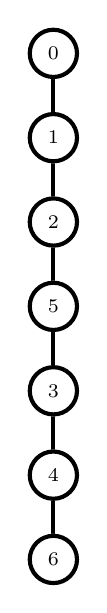
\begin{tikzpicture}[scale=0.45,line width = 1.5pt]
\draw [] (16.6667,32.14) -- (16.6667,29.76);
\draw [] (16.6667,29.76) -- (16.6667,27.38);
\draw [] (16.6667,27.38) -- (16.6667,25);
\draw [] (16.6667,25) -- (16.6667,22.6167);
\draw [] (16.6667,22.6167) -- (16.6667,20.2367);
\draw [] (16.6667,20.2367) -- (16.6667,17.8567);
\filldraw[color=white] (16.6667,32.14) circle [radius = 0.666667cm];
\draw (16.6667,32.14) circle [radius = 0.666667cm];
\draw (16.6667,32.14) node{{\scriptsize 0}};
\filldraw[color=white] (16.6667,29.76) circle [radius = 0.666667cm];
\draw (16.6667,29.76) circle [radius = 0.666667cm];
\draw (16.6667,29.76) node{{\scriptsize 1}};
\filldraw[color=white] (16.6667,27.38) circle [radius = 0.666667cm];
\draw (16.6667,27.38) circle [radius = 0.666667cm];
\draw (16.6667,27.38) node{{\scriptsize 2}};
\filldraw[color=white] (16.6667,25) circle [radius = 0.666667cm];
\draw (16.6667,25) circle [radius = 0.666667cm];
\draw (16.6667,25) node{{\scriptsize 5}};
\filldraw[color=white] (16.6667,22.6167) circle [radius = 0.666667cm];
\draw (16.6667,22.6167) circle [radius = 0.666667cm];
\draw (16.6667,22.6167) node{{\scriptsize 3}};
\filldraw[color=white] (16.6667,20.2367) circle [radius = 0.666667cm];
\draw (16.6667,20.2367) circle [radius = 0.666667cm];
\draw (16.6667,20.2367) node{{\scriptsize 4}};
\filldraw[color=white] (16.6667,17.8567) circle [radius = 0.666667cm];
\draw (16.6667,17.8567) circle [radius = 0.666667cm];
\draw (16.6667,17.8567) node{{\scriptsize 6}};
\end{tikzpicture}
